\chapter{Instalacion y Configuracion}

En este Capitulo Aparte de guiarle para realizar una exitosa implementacion
Local del Servidor de Produccion se hara referencia a cada una de las
Herramientas y librerias Utilizadas.

\section{Requerimientos}

\subsection{Requerimientos de Hardware}

Cualquier equipo que cumpla con las Caracteristicas para correr Windows 7 es suficiente
en terminos de requerimientos minimos de Hardware siempre y cuando el numero de usarios
esperados no sea alto, despues el resto dependera de sus necesidades.\\[0.5cm]

\subsection{Requerimientos de Hardware}

\begin{itemize}
    \item Procesador x86, x64 de 1 Ghz o superior.
    \item Memoria Ram 1 GB o Superior 
\end{itemize}


\subsection{Requerimientos de Software}


\begin{itemize}
    \item Apache 2.2
    \item PosgreSQL 9.2
    \item Python 2.7.x o Python 2.6.x
    \item Django 1.3.x o Superior
    \item PGAdmin
    \item psycopg2
    \item mod\_wsgi
    \item ReportLab
    \item easy\_thumbnails
    \item django\_extensions
    \item django\_cron
\end{itemize}


\section{Apache}

El servidor HTTP Apache es un servidor web HTTP de código abierto, para plataformas
Unix (BSD, GNU/Linux, etc.), Microsoft Windows, Macintosh y otras, que implementa
el protocolo HTTP/1.12 y la noción de sitio virtual. Cuando comenzó su desarrollo en 1995 se basó inicialmente
en código del popular NCSA HTTPd 1.3, pero más tarde fue reescrito por completo. Su nombre se
debe a que Behelendorf quería que tuviese la connotación de algo que es firme
y enérgico pero no agresivo, y la tribu Apache fue la última en rendirse al que pronto se
convertiría en gobierno de EEUU, y en esos momentos la preocupación de su grupo era que
llegasen las empresas y "civilizasen" el paisaje que habían creado los primeros ingenieros de internet.
Además Apache consistía solamente en un conjunto de parches a aplicar al servidor de NCSA.
En inglés, a patchy server (un servidor "parcheado") suena igual que Apache Server. 

El servidor Apache se desarrolla dentro del proyecto HTTP Server (httpd) de la
Apache Software Foundation.

Apache presenta entre otras características altamente configurables, bases de
datos de autenticación y negociado de contenido, pero fue criticado por la falta
de una interfaz gráfica que ayude en su configuración.\\[0.2cm]

Existen 2 caminos para instalar Apache La Primera Hacer una instalacion Limpia
de Apache, la 2da es cuando no se quiere trastear con tanta configuracion por lo que
opta por infraestructuras tipo WAMP, LAMP, WAPP, etc.

\subsection{Instalacion en Limpio}

Solo recomiendo este tipo de instalacion desde 0 para quienes ya poseen un conocimiento
avanzado en cuanto a manejo de servidores.

Descargamos de \url{Apache.org} la ultima version disponible, puedes utilizar el siguiente
vinculo: \url{http://www.apachehaus.com/cgi-bin/download.plx}. \\ 
Crea dos carpetas en la unidad C, la primera de nombre {\bfseries Apache} y la segunda
{\bfseries servidor}. Descomprime el archivo descargado y ejecútalo,
sigue los pasos de la instalación y de los datos que te piden solo escoge el
destino de la instalación, que será la carpeta que creaste en
{\bfseries C:\textbackslash Apache }, los otros datos déjalos de la forma
predeterminada para configurarlos más tarde.
El programa al instalarse crea un icono en el área de notificación que te
permitirá: iniciar, detener y reiniciar Apache; tienes que tener en cuenta que
cualquier cambio que hagas en el archivo de configuración no tendrá efecto
hasta que reinicies el servidor.

\subsection{Instalacion mediante WAMP, LAMP, MAMP, WAPP}

Existem una infinidad de Paquetes precompilados y configurados, con Apache, PHP, PosgreSQL o MySQL y mas.
Dichas infraestructuras suelen nombrarse como el acronomico de las herramientas que agrupan por ejemplo:\\[1cm]

\begin{itemize}
    \item {\large WAMP {\bfseries W}indows {\bfseries A}pache {\bfseries M}ySQL {\bfseries P}HP}
    \item {\large WAPP  {\bfseries W}indows {\bfseries A}pache {\bfseries P}osgreSQL {\bfseries P}HP}  
    \item {\large LAMP {\bfseries L}inux {\bfseries A}pache {\bfseries M}ySQL {\bfseries P}HP} 
    \item {\large MAMP {\bfseries M}ac OS {\bfseries A}pache {\bfseries M}ySQL {\bfseries P}HP}  
\end{itemize}


Algunas distribuciones mas usadas disponibles Para Windows son WAMP Server \url{http://www.wampserver.com/} (WAMP),
XAMPP \url{http://sourceforge.net/projects/xampp/} (WAMP + Perl), Bitnami \url{http://bitnami.com/stack/wapp} (WAPP)
solo nos resta elegir cualquiera de ellas e instalarlas, aparte de la ruta de instalacion nos pediran el usuario y
contraseña para acceder al motor de Base de Datos.

\subsection{Configuracion}

Toda la configuración para el funcionamiento de Apache se guarda en un archivo
de texto nombrado: {\bfseries httpd.conf} que se encuentra en la ruta
{\bfseries C:\textbackslash Apache \textbackslash conf } si realizamos una instalacion en limpio o
{\bfseries C:\textbackslash wamp \textbackslash bin \textbackslash  Apache \textbackslash conf } si
instalamos el paquete multiple preconfigurado no es necesario realizar este paso por lo
que lo podremos salta.\\

Al archivo {\bfseries httpd.conf} lo podemos editar en cualquier editor de texto como Notepad.

Buscamos la linea que dice

\begin{lstlisting}[style=consola, numbers=none]
    Listem LocalHost:80
\end{lstlisting}

y la Cambiamos por:

\begin{lstlisting}[style=consola, numbers=none]
    Listem 80
\end{lstlisting}

Ahora buscamos la instruccion:

\begin{lstlisting}[style=consola, numbers=none]
    DocumentRoot "C:\xxxxxxxx"
\end{lstlisting}

y la Cambiamos por:

\begin{lstlisting}[style=consola, numbers=none]
    DocumentRoot "C:\Servidor"
\end{lstlisting}

Recordar que al inicio de la instalacion creamos una Carpeta llamada Servidor en
la unidad C. Por ultimo solo nos queda reiniciar el servidor Apache e introducir
la siguiente direccion \url{http://127.0.0.1} si nos aparece una pagina
{\bfseries It's Work!} felicidades Apache esta Funcionando.


\section{PosgreSQL}

PostgreSQL es un gestor de base de datos relacional que puede correr tanto bajo
sistemas operativos Windows como en distribuciones Linux como Red Hat, Suse,
Centos, etc.

Como muchos otros proyectos de código abierto, el desarrollo de PostgreSQL
no es manejado por una empresa y/o persona, sino que es dirigido por una comunidad
de desarrolladores que trabajan de forma desinteresada, altruista, libre y/o
apoyados por organizaciones comerciales. Dicha comunidad es denominada
el PGDG (PostgreSQL Global Development Group).

El nombre hace referencia a los orígenes del proyecto como la base de datos
"post-Ingres", y los autores originales también desarrollaron la base de datos Ingres.

El proyecto post-ingres pretendía resolver los problemas con el modelo de base
de datos relacional que habían sido aclarados a comienzos de los años 1980. El
principal de estos problemas era la incapacidad del modelo relacional de
comprender "tipos", es decir, combinaciones de datos simples que conforman una
única unidad. Actualmente estos son llamados objetos. Se esforzaron en introducir
la menor cantidad posible de funcionalidades para completar el soporte de tipos.
Estas funcionalidades incluían la habilidad de definir tipos, pero también
la habilidad de describir relaciones - las cuales hasta ese momento eran
ampliamente utilizadas pero mantenidas completamente por el usuario. En Postgres
la base de datos «comprendía» las relaciones y podía obtener información de
tablas relacionadas utilizando reglas. Postgres usó muchas ideas de Ingres
pero no su código.

\subsection{Instalacion}

La versión de PostgreSQL que he utilizado durante el desarrollo del sistema es
la 9.2.x, quisas cuando leas esto haya salido una nueva version la cual no deberia
generar inconvenientes ademas de que es posible que el proceso de instalación
pueda variar.\\[0.2cm]
 
El primer paso es descargar el instalador de PostgreSQL para Windows,
lo puedes descargar desde el enlace siguiente
\url{http://www.postgresql.org/download/windows}, nos bajara un instalador similar
a {\bfseries postgresql-9.2.3-rc1-windows.exe} lo ejecutamos como administrador.\\[0.2cm]

Si tenemos activado el control de cuentas de usuario nos mostrará una advertencia
con el texto "¿Desea permitir que este programa realice cambios en el equipo?",
pulsaremos "Sí" para continuar con la instalación de PostgreSQL.\\[0.2cm]

Indicaremos la carpeta de instalación de PostgreSQL, donde se guardarán los
ejecutables, librerías y ficheros de configuración de PostgreSQL en mi caso el
directorio es {\bfseries C: \textbackslash PosgreSQL \textbackslash 9.2 },
Indicaremos también la carpeta donde se guardarán los datos por defecto
de PostgreSQL {\bfseries C: \textbackslash psql-data }.\\[0.2cm]

Solo nos queda introducir la contraseña para el superusuario "postgres" que
será con el que iniciemos sesión para administrar la base de datos, despues
podremos crear otros usuarios si es necesario. Ademas introduciremos el puerto
de escucha para la conexión con el servidor PostgreSQL, por defecto el 5432.\\[0.2cm]

Seleccionaremos la configuración regional y comenzara la instalacion, con esto
PosgreSQL quedara instalado. Si tenemos algún cortafuegos (firewall) deberemos
abrir el puerto 5432.

\subsection{Creacion de la Base de Datos}

Junto con la Instalacion de PosgreSQL se instala el PGAdmin III que es una Heramienta
GUI para administrar el motor de base de Datos. Iniciamos el Programa,
desplegaremos "Server Groups", dentro desplegaremos "Servidores" y dentro de
éste pulsaremos con el botón derecho del ratón sobre "PostgreSQL 9.0 (localhost:5432),
en el menú emergente seleccionaremos "Conectar".

Introduciremos la contraseña para el superusuario postgres
(la contraseña introducida en la instalación).

Pulsaremos con el botón derecho del ratón sobre "Bases de datos", seleccionaremos
"Nueva Base de Datos", en la pestaña "Propiedades" introduciremos los
siguientes datos:

\begin{itemize}
    \item Nombre: nombre de la base de datos, en nuestro caso "BDSem".
    \item Propietario: seleccionaremos el usuario creado anteriormente "posgres".
    \item Codificado: seleccionaremos UTF8.
    \item Tablespace: seleccionaremos el tablespace creado anteriormente "pg\_default".
    \item Colación: seleccionaremos "Spanish, Argentina".
    \item Tipo carácter: seleccionaremos "Spanish, Argentina".
\end{itemize}

Pulsaremos "OK" para crear la base de datos, con esto ya tendremos nuestra base
de datos aunque vacia, el resto como creacion de las Tablas correspondientes
nesesarias para el proyecto lo haremos mas adelante mediante Django.


\section{Python}

Django esta escrito puramente en Python, por lo que Obiamente Necesitaremos Instalar
Python. Python es un lenguaje de programación interpretado cuya filosofía hace
 hincapié en una sintaxis muy limpia y que favorezca un código legible.
 
Se trata de un lenguaje de programación multiparadigma, ya que soporta
orientación a objetos, programación imperativa y, en menor medida, programación
funcional. Es un lenguaje interpretado, usa tipado dinámico y es multiplataforma.

Es administrado por la Python Software Foundation. Posee una licencia de código
abierto, denominada Python Software Foundation License,1 que es compatible con
la Licencia pública general de GNU a partir de la versión 2.1.1, e
incompatible en ciertas versiones anteriores.

Python es un lenguaje de programación multiparadigma. Esto significa que más
que forzar a los programadores a adoptar un estilo particular de programación,
permite varios estilos: programación orientada a objetos, programación imperativa
y programación funcional. Otros paradigmas están soportados mediante el uso
de extensiones.

Python usa tipado dinámico y conteo de referencias para la administración
de memoria.

Una característica importante de Python es la resolución dinámica de nombres;
 es decir, lo que enlaza un método y un nombre de variable durante la ejecución
  del programa (también llamado enlace dinámico de métodos).
  
Otro objetivo del diseño del lenguaje es la facilidad de extensión. Se pueden
escribir nuevos módulos fácilmente en C o C++. Python puede incluirse en
aplicaciones que necesitan una interfaz programable.

Aunque la programación en Python podría considerarse en algunas situaciones
hostil a la programación funcional tradicional del Lisp, existen bastantes
analogías entre Python y los lenguajes minimalistas de la familia Lisp como
puede ser Scheme.

\subsection{La Filosofia detras de Python}
Los usuarios de Python se refieren a menudo a la Filosofía Python que es bastante
análoga a la filosofía de Unix. El código que sigue los principios de Python de
legibilidad y transparencia se dice que es "pythonico". Contrariamente, el
código opaco u ofuscado es bautizado como "no pythonico" ("unpythonic" en inglés).

Estos principios fueron famosamente descritos por el desarrollador de Python Tim
Peters en El Zen de Python, algunos de ellos son:

\begin{itemize}
    \item Bello es mejor que feo.
    \item Explícito es mejor que implícito.
    \item Simple es mejor que complejo.
    \item Complejo es mejor que complicado.
    \item Plano es mejor que anidado.
    \item Disperso es mejor que denso.
    \item La legibilidad cuenta.
    \item Los casos especiales no son tan especiales como para quebrantar las reglas.
    \item Aunque lo práctico gana a la pureza.
    \item Los errores nunca deberían dejarse pasar silenciosamente.
    \item A menos que hayan sido silenciados explícitamente.
    \item Frente a la ambigüedad, rechaza la tentación de adivinar.
    \item Debería haber una y preferiblemente sólo una manera obvia de hacerlo.
    \item Aunque esa manera puede no ser obvia al principio a menos que usted sea holandés.15
    \item Ahora es mejor que nunca.
    \item Aunque nunca es a menudo mejor que ya mismo.
    \item Si la implementación es difícil de explicar, es una mala idea.
    \item Si la implementación es fácil de explicar, puede que sea una buena idea.
    \item Los espacios de nombres (namespaces) son una gran idea ¡Hagamos más de esas cosas!
\end{itemize}


\subsection{Baterias Incluidas}

Python tiene una gran biblioteca estándar, usada para una diversidad de tareas.
Esto viene de la filosofía "pilas incluidas" ("batteries included") en referencia
a los módulos de Python. Los módulos de la biblioteca estándar pueden mejorarse por
módulos personalizados escritos tanto en C como en Python. Debido a la gran
variedad de herramientas incluidas en la biblioteca estándar, combinada con la
habilidad de usar lenguajes de bajo nivel como C y C++, los cuales son capaces
de interactuar con otras bibliotecas, {\bfseries Python es un lenguaje que combina su clara
sintaxis con el inmenso poder de lenguajes menos elegantes}.

\subsection{Implementaciones}

En la actualidad existen diversas implementaciones de Python

\begin{itemize}
    \item {\bfseries CPython} es la implementación original, disponible para varias plataformas en el sitio oficial de Python.
    \item {\bfseries IronPython} es la implementación para .NET
    \item {\bfseries Stackless Python} es la variante de CPython que trata de no usar el stack de C \url{www.stackless.com}
    \item {\bfseries Jython} es la implementación hecha en Java
    \item {\bfseries Pippy} es la implementación realizada para Palm \url{pippy.sourceforge.net}
    \item {\bfseries PyPy} es una implementación de Python escrita en Python y optimizada mediante JIT \url{pypy.org}
\end{itemize}

\subsection{Instalacion}

Para este proyecto se utilizo CPython pero no la version Oficial url{http://www.python.org}
sino la que distribuye Active State \url{http://www.activestate.com} llamada
{\bfseries Active Python} la cual provee caracteristicas adicionales a version oficial,
podremos descargar la ultima version desde \url{http://www.activestate.com/activepython/downloads}
aunque se recomienda instalar la version 2.7.x para evitar cualquier posible problema.

\subsection{Probando Python}
Para probar que la instalacion haya sido correcta abriremos la Terminal "cmd.exe"
y escribiremos:

\begin{lstlisting}[style=consola, numbers=none]
    python
\end{lstlisting} 

Si todo va bien nos debera aparecer algo similar a:

\begin{figure}[h]
    \centering
    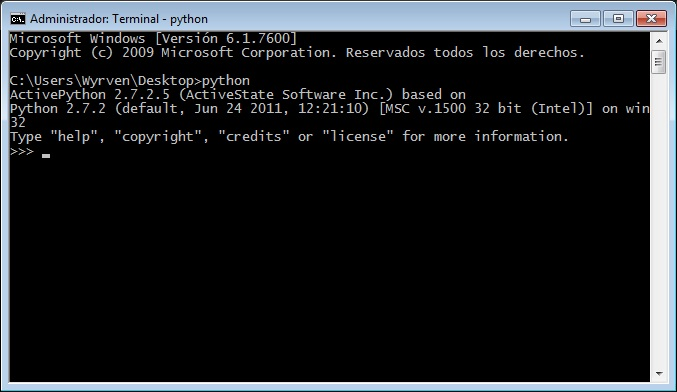
\includegraphics[scale=0.7]{resourse/consola-python.jpg}
    \caption{Ejecutando Python en la Terminal}
    \label{fig:01}
\end{figure}    

En caso contrario deberias revisar que la ruta de Python este dentro de la variable
 PATH del sistema.




